
\documentclass[11pt]{report}

\textheight=25.5cm \textwidth=18.5cm \topmargin=-3cm
\oddsidemargin=-1.5cm
\parindent=0mm

%\usepackage[spanish]{babel}
%\usepackage[latin1]{inputenc}
\usepackage[pdftex]{graphicx}

\usepackage{amsmath}
\usepackage{amsfonts}
\usepackage{amssymb}

\usepackage{tikz}
\usetikzlibrary{arrows}
\usetikzlibrary{babel}

\usepackage{amsthm}
\theoremstyle{definition}
\newcommand{\sen}{\mathrm{sen}}
\newtheorem*{comentario}{Comentario}
\newtheorem{definicion}{Definici\'on}
\newtheorem{teorema}{Teorema}
\newtheorem{corolario}{Corolario}
\newtheorem{problema*}{Problema}
\newtheorem{ejemplo}{Ejemplo}
\newtheorem{problema}{Problema}
\newtheorem{proposicion}{Proposici\'on}
\newtheorem{observacion}{Observaci\'on}
\newtheorem{ejercicio}{Ejercicio}
\newenvironment{solucion}{\begin{proof}[Solución]\small}{\end{proof}}

\pagestyle{empty}

\begin{document}


%\newpage
\begin{center}
\textbf{Entrenamiento para Olimpiadas de Matemáticas
\\EXAMEN: ANGLE CHASING\\
17 Marzo 2022}
\end{center}


\begin{problema}
 En la figura se muestra un cuadril\'atero $ABCD$. Si $BC=AD$, ?`cu\'anto mide el \'angulo $ADC$?

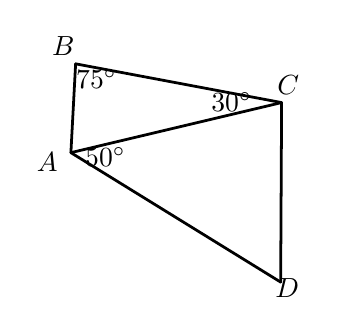
\begin{tikzpicture}[line cap=round,line join=round,>=triangle 45,x=0.6cm,y=0.6cm]
\draw [line width=1.pt] (1.76,-3.14)-- (-2.68,-0.4);
\draw [line width=1.pt] (1.76,-3.14)-- (1.78,0.66);
\draw [line width=1.pt] (1.78,0.66)-- (-2.58,1.48);
\draw [line width=1.pt] (-2.58,1.48)-- (-2.68,-0.4);
\draw [line width=1.pt] (-2.68,-0.4)-- (1.78,0.66);
\draw[color=black] (-3.18,-0.59) node {$A$};
\draw[color=black] (-1.95,-0.50) node {$50^{\circ}$};
\draw[color=black] (-2.84,1.85) node {$B$};
\draw[color=black] (-2.14,1.15) node {$75^{\circ}$};
\draw[color=black] (1.92,1.03) node {$C$};
\draw[color=black] (0.72,0.67) node {$30^{\circ}$};
\draw[color=black] (1.9,-3.27) node {$D$};
\end{tikzpicture}

%(P23 Nivel Ol\'impico MatPreolimpicasMLPS)
\end{problema}

\begin{problema}
En la figura $ABCD$ es un cuadrado y $OBC$ es un tri\'angulo equil\'atero. ?`Cu\'anto
mide el \'angulo $\angle OAC$?


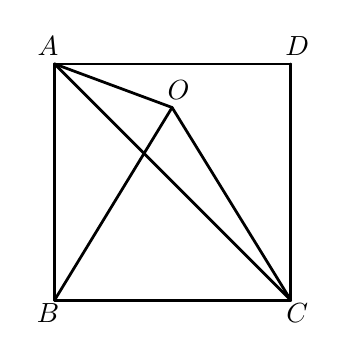
\begin{tikzpicture}[line cap=round,line join=round,>=triangle 45,x=4.0*.75cm,y=4.0*.75cm]
\draw [line width=1.pt] (0.,1.)-- (0.,0.);
\draw [line width=1.pt] (0.,0.)-- (1.,0.);
\draw [line width=1.pt] (1.,0.)-- (1.,1.);
\draw [line width=1.pt] (1.,1.)-- (0.,1.);
\draw [line width=1.pt] (0.49753086419753084,0.8155555555555556)-- (0.,0.);
\draw [line width=1.pt] (0.49753086419753084,0.8155555555555556)-- (1.,0.);
\draw [line width=1.pt] (0.49753086419753084,0.8155555555555556)-- (0.,1.);
\draw [line width=1.pt] (0.,1.)-- (1.,0.);
\draw[color=black] (-0.027407407407407193,1.074320987654321) node {$A$};
\draw[color=black] (-0.027407407407407193,-0.0548148148148148) node {$B$};
\draw[color=black] (1.0269135802469138,-0.0548148148148148) node {$C$};
\draw[color=black] (1.0269135802469138,1.074320987654321) node {$D$};
\draw[color=black] (0.5251851851851852,0.8886419753086421) node {$O$};
\end{tikzpicture}
%\\(P53 Nivel Ol\'impico MatPreolimpicasMLPS)

\end{problema}

\begin{problema}
Los \'angulos en las esquinas de la estrella son los marcados. ?`Cu\'anto
vale $x?$

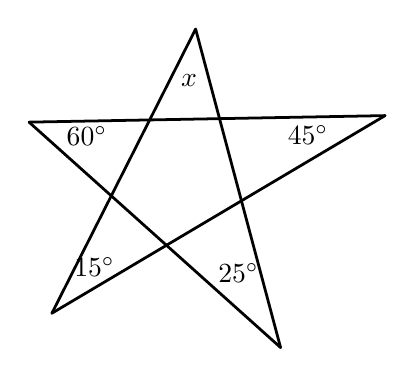
\begin{tikzpicture}[line cap=round,line join=round,>=triangle 45,x=3.5cm,y=3.5cm]
\draw [line width=1.pt] (0.9044444444444447,0.03135802469135847)-- (-0.008148148148148491,0.8491358024691361);
\draw [line width=1.pt] (0.9044444444444447,0.03135802469135847)-- (0.5962962962962963,1.1869135802469137);
\draw [line width=1.pt] (0.07481481481481453,0.1558024691358029)-- (0.5962962962962963,1.1869135802469137);
\draw [line width=1.pt] (0.07481481481481453,0.1558024691358029)-- (1.2837037037037042,0.8728395061728398);
\draw [line width=1.pt] (1.2837037037037042,0.8728395061728398)-- (-0.008148148148148491,0.8491358024691361);
\draw[color=black] (0.751851851851852,0.30172839506172877) node {$25^{\circ}$};
\draw[color=black] (0.2018518518518516,0.7987654320987657) node {$60^{\circ}$};
\draw[color=black] (1.0040740740740746,0.8020987654320991) node {$45^{\circ}$};
\draw[color=black] (0.5725925925925927,1.0013580246913583) node {$x$};
\draw[color=black] (0.22925925925925905,0.32469135802469173) node {$15^{\circ}$};
\end{tikzpicture}
%\\(P41 Nivel Estudiante MatPreolimpicasMLPS)

\end{problema}


\begin{problema}
En la figura, los puntos $A,P,Q$ y $R$ est\'an sobre la circunferencia con centro
$C$; $ABCD$ es un cuadrado; la recta $PR$ pasa por $B$ y $D$; la recta $QR$ pasa por $C$.
Determinar el \'angulo $\angle PQR$.

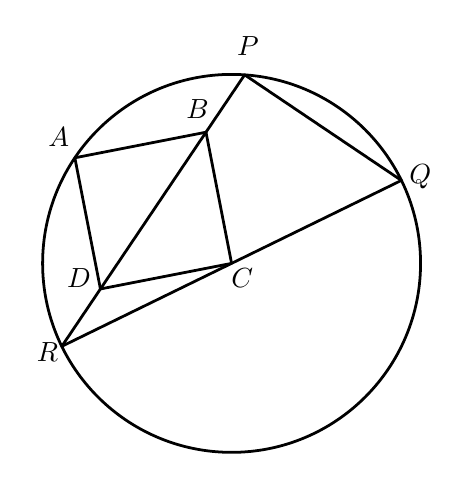
\begin{tikzpicture}[line cap=round,line join=round,>=triangle 45,x=3.0*0.8cm,y=3.0*0.8cm]
\draw [line width=1.pt] (0.,0.) circle (3.0*0.8cm);
\draw [line width=1.pt] (0.,0.)-- (-0.13542605358503557,0.6940171352426272);
\draw [line width=1.pt] (-0.13542605358503557,0.6940171352426272)-- (-0.8294431888276628,0.5585910816575916);
\draw [line width=1.pt] (-0.8294431888276628,0.5585910816575916)-- (-0.6940171352426272,-0.13542605358503557);
\draw [line width=1.pt] (0.,0.)-- (-0.6940171352426272,-0.13542605358503557);
\draw [line width=1.pt] (-0.8984756614567335,-0.43902333169193314)-- (0.8984756614567335,0.43902333169193314);
\draw [line width=1.pt] (0.8984756614567335,0.43902333169193314)-- (0.06903247262907086,0.9976144133495249);
\draw [line width=1.pt] (-0.8984756614567335,-0.43902333169193314)-- (0.06903247262907086,0.9976144133495249);
\draw[color=black] (0.057037037037036734,-0.07827160493827115) node {$C$};
\draw[color=black] (-0.9148148148148156,0.6683950617283954) node {$A$};
\draw[color=black] (-0.808148148148149,-0.07827160493827115) node {$D$};
\draw[color=black] (-0.18,0.8165432098765434) node {$B$};
\draw[color=black] (0.08666666666666636,1.1483950617283951) node {$P$};
\draw[color=black] (0.9992592592592594,0.4609876543209879) node {$Q$};
\draw[color=black] (-0.974074074074075,-0.46938271604938214) node {$R$};
\end{tikzpicture}

%(P29 Nivel Semifinal MatPreolimpicasMLPS)
\end{problema}


\newpage

\begin{problema}
Sea $ABC$ un tri\'angulo y $AD$ la altura sobre el lado $BC$. Tomando a $D$ como
centro y a $AD$ como radio, se traza una circunferencia que corta a la recta $AB$ en
$P$, y corta a la recta $AC$ en $Q$. Muestra que el tri\'angulo $AQP$ es semejante
al tri\'angulo $ABC$.

%\includegraphics[width=0.45\textwidth]{figuras/P1_omm_2009_1}
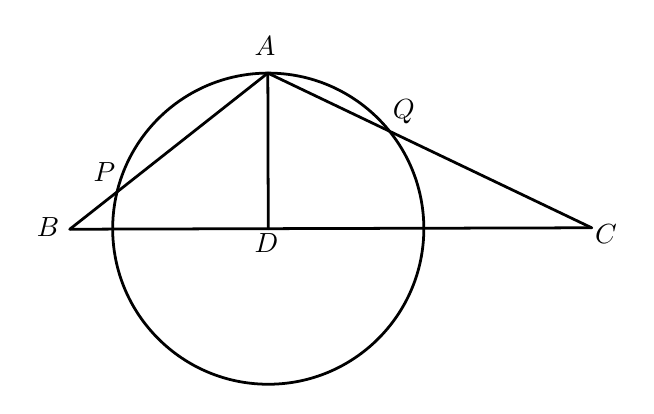
\begin{tikzpicture}[line cap=round,line join=round,>=triangle 45,x=4*1.0cm,y=4*1.0cm]
\draw [line width=1.pt] (0.863807405686497,-0.14503467816191534) circle (4*0.4939628904042216cm);
\draw [line width=1.pt] (0.23362602737072305,-0.14678033294949364)-- (1.8905714038434012,-0.14219045656037266);
\draw [line width=1.pt] (0.23362602737072305,-0.14678033294949364)-- (0.862439092680299,0.3489263170755732);
\draw [line width=1.pt] (0.862439092680299,0.3489263170755732)-- (1.8905714038434012,-0.14219045656037266);
\draw [line width=1.pt] (0.862439092680299,0.3489263170755732)-- (0.863807405686497,-0.14503467816191534);
\draw[color=black] (0.853259339902057,0.4338390302743115) node {$A$};
\draw[color=black] (0.16477788153390815,-0.13989551836581215) node {$B$};
\draw[color=black] (1.936470167734611,-0.1628449003114171) node {$C$};
\draw[color=black] (0.857849216291178,-0.19038415864614305) node {$D$};
\draw[color=black] (0.34378306070962683,0.03451978442078544) node {$P$};
\draw[color=black] (1.2938874732576722,0.227294592763867) node {$Q$};
\end{tikzpicture}

%(P1 OMM 2009)%23aOMM
\end{problema}

\begin{problema}
Sean $A$ y $B$ dos puntos fijos en el plano y sea $\mathcal{L}$ una recta que
pasa por $A$ pero no por $B$. Para $P$ y $Q$ puntos de $\mathcal{L}$ (distintos de $A$)
sean $O_P$ y $O_Q$ los centros de las circunferencias circunscritas a $APB$ y $AQB$,
respectivamente. Demostrar que los \'angulos $\angle O_P PB$ y $\angle O_Q QB$ son
iguales.


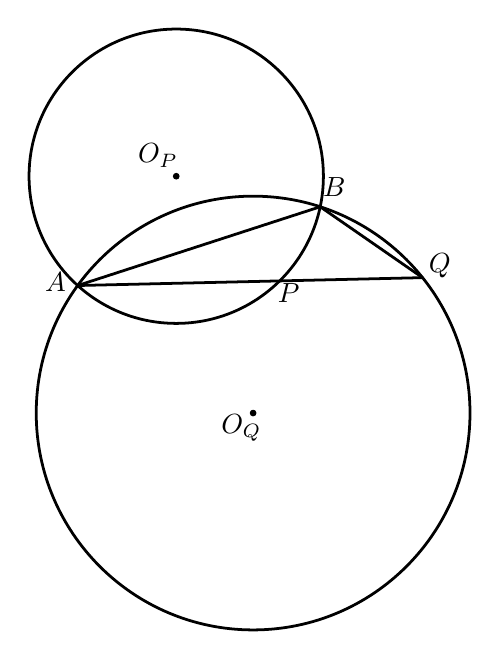
\begin{tikzpicture}[line cap=round,line join=round,>=triangle 45,x=1.0cm,y=1.0cm]
\draw [line width=1.pt] (0.04,0.58)-- (4.42,0.68);
\draw [line width=1.pt] (1.2916624952126992,1.9680795147448864) circle (1.8690702879176266cm);
\draw [line width=1.pt] (2.2681139489194497,-1.0393909626719047) circle (2.7544362144280745cm);
\draw [line width=1.pt] (0.04,0.58)-- (3.12,1.58);
\draw [line width=1.pt] (3.12,1.58)-- (4.42,0.68);
\draw[color=black] (-0.24,0.63) node {$A$};
\draw[color=black] (3.3,1.83) node {$B$};
\draw[color=black] (4.64,0.83) node {$Q$};
\draw[color=black] (2.72,0.49) node {$P$};
\draw [fill=black] (2.2681139489194497,-1.0393909626719047) circle (1.0pt);
\draw[color=black] (2.12,-1.23) node {$O_Q$};
\draw [fill=black] (1.2916624952126992,1.9680795147448864) circle (1.0pt);
\draw[color=black] (1.06,2.23) node {$O_P$};
\end{tikzpicture}

%(P14 Nivel Final MatPreolimpicasMLPS)
\end{problema}

\begin{problema}
Supongamos que $M$ y $N$ son los puntos de tangencia de una circunferencia inscrita
con los lados $BC$ y $BA$ del tri\'angulo $ABC$; $K$, el punto de intersecci\'on de la
bisectriz del \'angulo $A$ con la recta $MN$. Demostrar que $\angle AKC=90^\circ$.

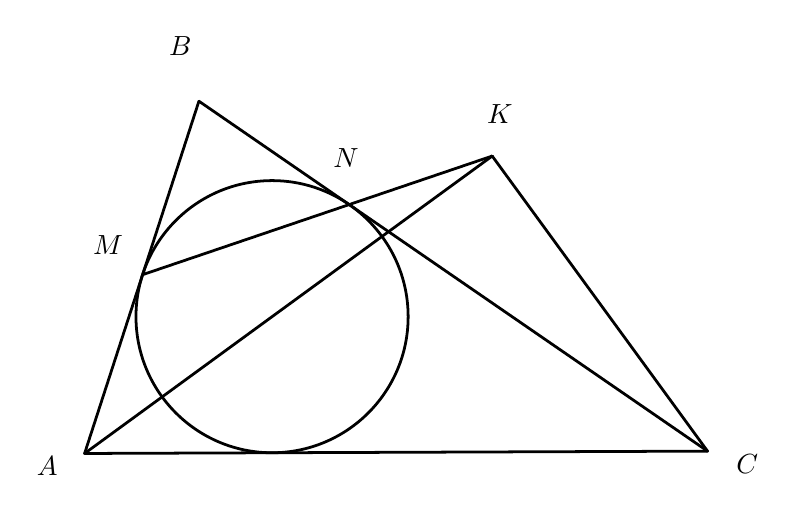
\begin{tikzpicture}[line cap=round,line join=round,>=triangle 45,x=5cm,y=5cm]
\draw [line width=1.pt] (-0.3992592592592598,-0.36567901234567846)-- (-0.10888888888888928,0.529135802469136);
\draw [line width=1.pt] (-0.10888888888888928,0.529135802469136)-- (1.1829629629629632,-0.3597530864197525);
\draw [line width=1.pt] (1.1829629629629632,-0.3597530864197525)-- (-0.3992592592592598,-0.36567901234567846);
\draw [line width=1.pt] (0.07687326819735947,-0.018246935369252804) circle (5*0.34564638483012994cm);
\draw [line width=1.pt] (-0.3992592592592598,-0.36567901234567846)-- (0.6360369217846424,0.3897726355122104);
\draw [line width=1.pt] (-0.25189618744067716,0.08843984162587176)-- (0.6360369217846424,0.3897726355122104);
\draw [line width=1.pt] (0.6360369217846424,0.3897726355122104)-- (1.1829629629629632,-0.3597530864197525);
\draw[color=black] (-0.49407407407407467,-0.398271604938271) node {$A$};
\draw[color=black] (1.2837037037037042,-0.3923456790123451) node {$C$};
\draw[color=black] (-0.1562962962962967,0.6683950617283954) node {$B$};
\draw[color=black] (-0.34,0.16469135802469176) node {$M$};
\draw[color=black] (0.26444444444444426,0.3839506172839509) node {$N$};
\draw[color=black] (0.6555555555555556,0.4965432098765435) node {$K$};
\end{tikzpicture}

%(SHARIGUIN I.255)
\end{problema}

\newpage

\begin{problema}
En el tri\'angulo is\'osceles $ABC$ se tiene que $\angle C>90$. Sean $O$ el circuncentro del tri\'angulo,
$I$ el incentro y $D$ el punto sobre $BC$ de tal manera que las l\'ineas $OD$ y $BI$ son perpendiculares.
Prueba que $ID$ y $AC$ son paralelas.

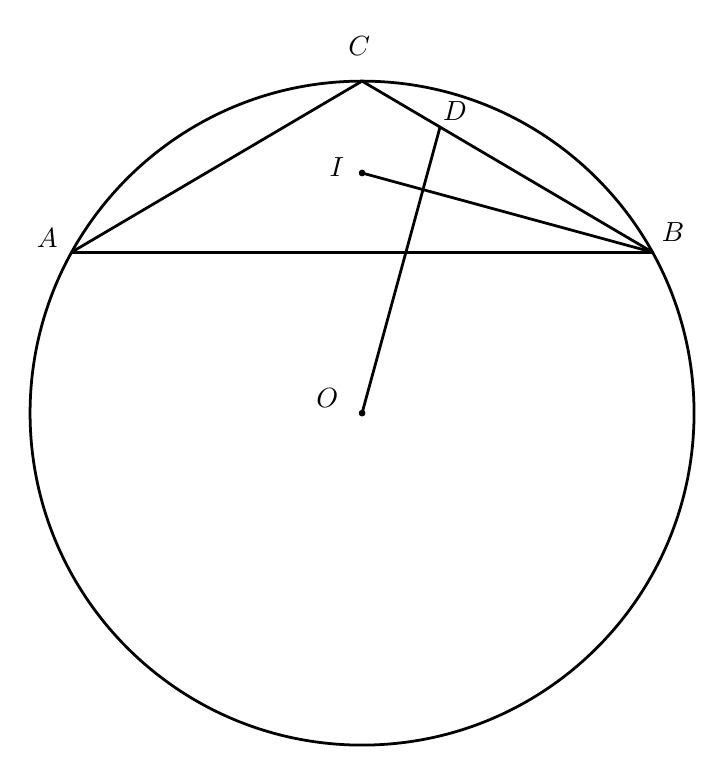
\begin{tikzpicture}[line cap=round,line join=round,>=triangle 45,x=4*1.3cm,y=4*1.3cm]
\draw [line width=1.pt] (0.7499871211468343,-0.879578056618647) circle (4*0.81082562228421*1.3cm);
\draw [line width=1.pt] (0.04085121902764139,-0.4864311857444469)-- (1.4591230232660277,-0.4864311857444469);
\draw [line width=1.pt] (0.04085121902764139,-0.4864311857444469)-- (0.7499871211468345,-0.06875243433443678);
\draw [line width=1.pt] (0.7499871211468345,-0.06875243433443678)-- (1.4591230232660277,-0.4864311857444469);
\draw [line width=1.pt] (0.7499871211468343,-0.879578056618647)-- (0.9404463682306589,-0.18093231449384145);
\draw [line width=1.pt] (1.4591230232660277,-0.4864311857444469)-- (0.7499871211468344,-0.2931121946532464);
\draw[color=black] (-0.018817174030931506,-0.45200711282603945) node {$A$};
\draw[color=black] (1.5096116635463588,-0.43823748365867643) node {$B$};
\draw[color=black] (0.7431023065631532,0.01616027886430148) node {$C$};
\draw [fill=black] (0.7499871211468343,-0.879578056618647) circle (1.0pt);
\draw[color=black] (0.6650744079480964,-0.8421466059013235) node {$O$};
\draw [fill=black] (0.7499871211468344,-0.2931121946532464) circle (1.0pt);
\draw[color=black] (0.6880237898937013,-0.2775918100394419) node {$I$};
\draw[color=black] (0.9771860024083238,-0.14153601280932821) node {$D$};
\end{tikzpicture}

%(PRE 1999)
\end{problema}



\begin{problema}
En el tri\'angulo $ABC$ se tiene que $AB=AC$. Una circunferencia es tangente internamente
al circunc\'icrulo de $ABC$ y tambi\'en a los lados $AB$ y $AC$ en los puntos $P$ y $Q$,
respectivamente. Demuestre que el punto medio de $PQ$ es el incentro de $ABC$.

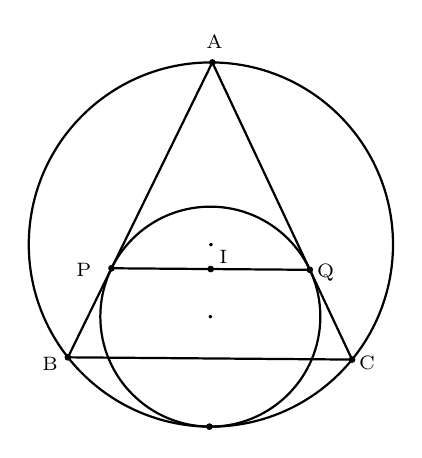
\begin{tikzpicture}[line cap=round,line join=round,>=triangle 45,x=0.5cm,y=0.5cm]
%\clip(-0.48,-0.266) rectangle (37.646,19.622);
\draw [line width=0.8pt] (6.714,7.522) circle (2.794086612830748*0.5cm);
\draw [line width=0.8pt] (6.728420782498949,9.353439377366428) circle (4.62558276405144*0.5cm);
\draw [line width=0.8pt] (6.764841564997898,13.978878754732857)-- (10.31447303697543,6.431754052891199);
\draw [line width=0.8pt] (10.31447303697543,6.431754052891199)-- (3.096805231809961,6.48858608285313);
\draw [line width=0.8pt] (3.096805231809961,6.48858608285313)-- (6.764841564997898,13.978878754732857);
\draw [line width=0.8pt] (4.204645231300158,8.750844434744842)-- (9.2423943084945,8.711177119176382);
\begin{scriptsize}
\draw [fill=black] (6.692,4.728) circle (1.0pt);
\draw [fill=black] (6.714,7.522) circle (0.5pt);
\draw [fill=black] (6.764841564997898,13.978878754732857) circle (1.0pt);
\draw[color=black] (6.824,14.507) node {A};
\draw [fill=black] (9.2423943084945,8.711177119176382) circle (1.0pt);
\draw[color=black] (9.64,8.633) node {Q};
\draw [fill=black] (4.204645231300158,8.750844434744842) circle (1.0pt);
\draw[color=black] (3.502,8.721) node {P};
\draw [fill=black] (6.728420782498949,9.353439377366428) circle (0.5pt);
\draw [fill=black] (3.096805231809961,6.48858608285313) circle (1.0pt);
\draw[color=black] (2.644,6.323) node {B};
\draw [fill=black] (10.31447303697543,6.431754052891199) circle (1.0pt);
\draw[color=black] (10.696,6.345) node {C};
\draw [fill=black] (6.7235197698973295,8.731010776960613) circle (1.0pt);
\draw[color=black] (7.044,9.029) node {I};
\end{scriptsize}
\end{tikzpicture}


%(P4 IMO 1978)
\end{problema}

\begin{problema}
Sea $P$ un punto en el interior del triángulo $ABC$ (con $CA \neq CB$). Las líneas $AP$, $BP$ y $CP$ se intersectan con el circuncírculo $\Gamma$ en $K$, $L$, y $M$, respectivamente. La tangente a $\Gamma$ en $C$ intersecta a $AB$ en $S$. Muestra que si $SC = SP$ entonces $MK = ML$.

%[P4 IMO 2010]
\end{problema}

\begin{problema}
Sean $\mathcal{C}_1$ y $\mathcal{C}_2$ dos circunferencias tangentes externamente en 
$S$ tales que el radio de $\mathcal{C}_2$ es el triple del radio de $\mathcal{C}_1$. Sea 
$l$ una recta que es tangente a $\mathcal{C}_1$ en $P$ y tangente a $\mathcal{C}_2$ en $Q$,
con $P$ y $Q$ distintos de $S$. Sea $T$ el punto en $\mathcal{C}_2$ tal que $TQ$ es di\'ametro 
de $\mathcal{C}_2$ y sea $R$ la intersecci\'on de la bisectriz de $\angle SQT$ con el segmento 
$ST$. Demuestra que $QR = RT$.

%(P1 OMM 2016)
\end{problema}

\begin{problema}
Considera un cuadrilátero convexo $ABCD$. El punto $P$ se encuentra en el interior de $ABCD$. Se cumplen las siguientes proporciones:
\[\angle PAD:\angle PBA:\angle DPA=1:2:3=\angle CBP:\angle BAP:\angle BPC\]
Muestra que las tres líneas siguientes concurren en un punto: las bisectrices interiores de los ángulos $\angle ADP$ y $\angle PCB$ y la mediatriz de $AB$. 

%[P1 IMO2020]
\end{problema}

\end{document}
